% TODO finish part 2.3
% TODO finish part 3
% TODO finish part 4

\documentclass[british,11pt,a4paper]{article}
\usepackage[british]{babel}
\usepackage[margin=1in, bottom=1in, top=1in, footskip=0.25in]{geometry}
\usepackage[titletoc]{appendix}
\usepackage{fancyhdr}
\usepackage{mathtools}
\usepackage[numbers]{natbib}
\usepackage{pgfplotstable,filecontents}
\usepackage{hyperref}
\usepackage{booktabs}
\usepackage{wrapfig}
\usepackage{listings}
\usepackage{color}
\usepackage{graphicx}
\usepackage{siunitx}
\usepackage{tikz} % To generate the plot from csv
\usepackage{pgfplots}
\usepgfplotslibrary{statistics}

\pgfplotsset{compat=newest} % Allows to place the legend below plot
\usepgfplotslibrary{units} % Allows to enter the units nicely


\graphicspath{ {images/} }

\setcounter{secnumdepth}{2}
\setcounter{tocdepth}{2}
\renewcommand{\arraystretch}{1.2}
\renewcommand\thesection{\arabic{section}}
\renewcommand\thesubsection{\roman{subsection}.}
\renewcommand\thesubsubsection{}
\newcommand*{\Appendixautorefname}{appendix}
\pagestyle{fancy}
\fancyhf{}
\renewcommand{\headrulewidth}{0pt}
\lfoot{Exam no: Y0076159}
\cfoot{\thepage}
\lstset{
  language=Haskell,
  columns=fixed,
  breaklines=true,
  basicstyle=\ttfamily\footnotesize
  }

\usepackage[nottoc]{tocbibind}
\usepackage{csvsimple}

\begin{document}
\title{CTAP Open Assessment}
\author{Exam no: Y0076159}
\date{\today}
\maketitle
\tableofcontents
\clearpage
\section{Breaking Stream Ciphers}
\subsection{Implementation and Challenge}
The stream cipher implementation, found in \autoref{app:stream} (written in Python),
can be ran using the Python 2.7.6 compiler with the command \lstinline{python stream.py}. This will produce the
challenge 25 bit output of 3 Lfsrs with initial states 97, 975 and 6420:

1 0 1 0 1 0 1 1 1 0 1 0 1 1 0 0 0 0 0 0 1 0 0 1 1

\subsubsection{Code description}
The class \lstinline{Lfsr} implements an LFSR with a tap sequence, size and initial state. It contains 2 methods:
\lstinline{calc_tap}, which calculates the tap value for the current register value, and \lstinline{shift} which
calculates the tap value, shifts the register and outputs the register's value. The 3 LFSR's are combined using
\lstinline{combine_lfsr_outputs}, which uses a lookup table to implement the boolean operation.

\subsection{Cryptanalysis}
\subsubsection{Analysis}

\begin{center}
	\begin{tabular}{lllp{6.5cm}}\label{tab:streamattack} \\
		\toprule \\
		Linear func.                  & Walsh transform & Attack No & Attack description                                           \\
		\midrule \\
		\(R_3\) & 0 \\
		\(R_2\)                       & 0               &           &                                                              \\
		\(R_2 \oplus R_3\)            & 0               &           &                                                              \\
		\(R_1\)                       & -4              & 1         & No dependencies, has a single outlier agreement (see \autoref{app:lfsragreements} \\
		\(R_1 \oplus R_3\)            & -4              & 3         & Requires \(R_1\), attack with \(R_1 \oplus R_3 \oplus K\)    \\
		\(R_1 \oplus R_2\)            & 4               & 2         & Requires \(R_1\), attack with \(R_1 \oplus R_2 \oplus K\)    \\
		\(R_1 \oplus R_2 \oplus R_3\) & -4              &           &                                                              \\

		\bottomrule \\
	\end{tabular}
\end{center}
Using the Walsh transform displayed in \autoref{app:streamattack}, we can implement a divide-and-conquer strategy.
LFSR1 correlates quite strongly with the output (Walsh value of -4, 2 agreements and 6 disagreements resulting in a probability of 2/8 that it will agree with the function's output, with a bias of 0.25); this is reflected by the outlying value in the graph of sub-keys and their agreements with outputs in \autoref{app:lfsragreements}. As such, it can be brute-forced to obtain it's key value by iterating over the space of sub-keys, and finding the one with the highest agreement (sub-key value 27, with an agreement of 0.253).

The next attack targets \(R_1 \oplus R_2\), as it has a Walsh value of 4 (6 agreements and 2 disagreements resulting in a probability of 6/8, and a bias of -0.25). It is not feasible to brute-force this LFSR due to the lack of any outlying sub-key agreement.
The search space is reduced from \(O(n^{7} * n^{11})=O(n^{18})\) to \(O(n^7 + n^{11})=O(n^{11}))\) as we now know the key for LFSR1, allowing us to rapidly brute force the sub key for LFSR2 (value 1357, with agreement 0.247).

Finally LFSR3 can be attacked using \(R_1 \oplus R_3\), with a Walsh value of -4 (same agreements, disagreements, probability of correlation and bias as previous).
As LFSR1's key is known, the search space is also reduced for this attack from \(O(n^{7} * n^{13})=O(n^{20})\) to \(O(n^7 + n^{13})=O(n^{13}))\). This resulted in the sub-key for LFSR3 (value 7531, with agreement 0.245). This LFSR was also not brute-forcible due to a lack of outlying key agreements, as visible in the box-and-whisker plots in \autoref{app:lfsragreements}, where the biggest outlying agreement in LSFR3 is significantly closer to the median than the outlying agreement for LSFR1; this suggests a lower likelihood of the outlying key being correct.

Using this strategy, we have successfully attacked all 3 shift registers in a severely reduced search space (\(O(n^{7+11+13})>(O(n^{7}+n^{11}+n^{13})=O(n^{13}))\) (a reduction of 18 bits), resulting in the set of sub-keys: 27, 1357, and 7531.

\subsubsection{Attack Implementation}
The Python program which implements this attack loads a key-stream from \lstinline{stream.txt}, and begins by brute forcing the first register.
This is achieved by iterating over all possible keys, recording their agreement with the given data, and returning the key with the highest normalized agreement.
The next 2 LFSR's are then broken by iterating over each respective set of possible keys in combination with the output of LFSR1 using the previously known key.
This results in the set of initial states: \lstinline{lfsr1: 27, lfsr2: 1357, lfsr3: 7531}.

\subsection{Improvement}
The current function's key weakness is the correlation of a single shift register (LFSR1) with the output: this allows the key to be brute forced in \(O(n^7)\), followed by the other two keys in \(On^{11}\) and \(On^{13}\).
As such, the current function is not correlation immune to any significant order.
By changing the combination function's output to 1 0 0 1 0 1 1 0 (two bit flips on L001 and L101), we can ensure the function
is correlation immune to order 2, as the Walsh-Hadamard values for \(R_1\),
\(R_2\),  \(R_3\),  \(R_1 \oplus R_2\), \(R_1 \oplus R_3\) and \(R_1 \oplus R_3\), are now 0,
and therefore have no exploitable correlation exist other than all 3 registers combined; this is visible in the table below.

\begin{center}
	\begin{tabular}{@{}lll@{}}\label{tab:walsh2} \\
		Input & \(f\) & \(w\) \\
		\midrule \\
		000   & 1     & 0     \\
		001   & 0     & 0     \\
		010   & 0     & 0     \\
		011   & 1     & 0     \\
		100   & 0     & 0     \\
		101   & 1     & 0     \\
		110   & 1     & 0     \\
		111   & 0     & -8    \\
		\bottomrule \\
	\end{tabular}
\end{center}
This would restrict the attack vector to a combination of LFSR1, LFSR2 and LFSR3 simultaneously, with a Walsh-Hadamard value of -8 for \(R_1 \oplus R_2 \oplus R_3\); this is acceptable as exploiting
this would require iterating over the complete key-set \(O(n^{7+11+13}) = O(n^{31})\), causing the time complexity to be significantly higher than the previous \(O(n^{13}))\).
\clearpage
\section{Differential Cryptanalysis}
\subsection{Implementation and Challenge}
The block cipher found in \autoref{app:block} (written in Python),
can be ran using the Python 2.7.6 compiler with the command \lstinline{python block.py}. This will produce the
challenge output of 45858 (1011001100100010 in binary).
\subsection{Code description}
The block cipher is implemented using the \lstinline{do_4_rounds} method, which controls the execution of substitutions, permutations or combinations
of intermediary results with sub-keys dependent on the round. These sub-methods are implemented in \lstinline{do_substitution(), permute(), and combine_key()} respectively.
\subsection{Cryptanalysis}
\subsubsection{Analysis}
Following Hey's tutorial, a differential cryptanalysis attack was undertaken on
the S-box. The XOR table of differences was generated using \lstinline{calculate_xor_profiles()} in \autoref{app:blockattack}. This produced the difference distribution table found in \autoref{app:diff_distrib_tab}.
This indicated a number of high probability difference pairs:

\begin{center}
	\begin{tabular}{lll}\label{tab:diffpairs} \\
		\toprule \\
		$\triangle X$ & $\triangle Y$ & Difference \\
		1 & 3 & 8 \\
    	5 & 8 & 8 \\
    	8 & 14 & 8 \\
    	12 & 5 & 6 \\
    	13 & 6 & 6 \\
    	4 & 11 & 6 \\
    	9 & 13 & 6 \\
		\bottomrule \\
	\end{tabular}
\end{center}

Using as many of these high-probability difference pairs as possible a set of high probability paths (which go through a minimal amount of S-boxes) can be used to find pairs of plain-text differences and cipher-text differences. These are illustrated in \autoref{app:paths}, which were picked through trial-and-error to find paths with maximal probability which only impacted a single set of 4 bits, so as to avoid iterating over more than \(2^4\) bits per attack; as such, 4 consecutive \(O(2^4)\) attacks occurred to recover the 16 bit sub key. These paths could also have been obtained using Matsui's algorithm \cite{matsui}. 
\\ 
Using these paths, we were able to find a degree of certainty with which we can brute force the keys for 4-bit clusters to find the sub-key which maximally agrees with the provided plain-text/cipher-text pairs. This can be seen in the table below.

\begin{center}
	\begin{tabular}{llllll}\label{tab:pathprobabilities} \\
		\toprule \\
		Sub-key bits & $\triangle P$ & $\triangle U$ & Path probability &  Sub-key & Agreement with plain-text/cipher-text pairs\\
		1..4 & 12 & 12288 & 0.0234 & 0xD & 0.2083\\ 
		5..8 & 13 & 768 & 0.0059 & 0xD & 0.1181\\ 
		9..11 & 2 & 48 & 0.0078 & 0xD & 0.1627\\
		12..16 & 17 & 1 & 0.0039 & 0x5 & 0.0855\\ 
		\bottomrule \\
	\end{tabular}
\end{center}
As such, we were able to fully extract sub-key \(K_5\) with a value of \lstinline{0xDDD5}.
\subsubsection{Implementation}
As detailed above, the difference distribution table found in \autoref{app:diff_distrib_tab} was generated using \lstinline{calculate_xor_profiles()}, which simply iterated over every pair of possible 4 bit differences, and evaluated them against the configuration of the S-box. The list of differential pairs is then printed to console in descending probability of occurrence.
\\
Using the manually-found paths through the substitution/permutation network, the sub-key brute-forcing was implemented in the \lstinline{crack_section_subkey()} method which can be found in \autoref{app:blockattack}. It takes in $\triangle P$ and $\triangle U$ values, along with a mask and shift to indicate which group of 4 bits is attacked by the iteration. The data is then loaded from block.txt, and each possible 4-bit sub-key is iterated over each plain-text/cipher-text combination. Another plain-text/cipher-text combination is found by xor-ing the current plain-text with the requested difference, resulting in a second cipher-text. Both cipher-texts are then xor'd with the hypothetical sub-key (shifted to match the correct 4 bit cluster), and masked. They are then passed through the S-box in reverse, before being compared to the expected difference. 
\\
The list of potential sub-keys is then ordered by highest agreement, and the most promising key is returned.
\\
This attack is repeated 4 times to attack each 4 bit section of the sub-key, as visible in \lstinline{main()}.

{}
\subsection{Improvements}
The resilience of the cipher could be improved in two approaches. Firstly, the addition of additional rounds would significantly decrease the likelihood of finding high-probability paths through the substitution-permutation network. This could cause brute-forcing algorithms to produce hypothetical sub-key sections which are proportionally less agreeable to plain-text/cipher-text pairs than erroneous keys, and therefore less liable to have a superior agreement over other sub-key sections. This could however be overcome with the use of additional computational time and a larger set of plain-text/cipher-text pairs to improve the significance of the obtained statistics.
\\  
S-boxes present the other significant area for resilience; an S-box's strength can be seen as a combination of it's non-linearity (avoid the possibility of finding linear combinations of inputs which agree with linear combinations of subsets of outputs) and minimal autocorrelation (correlations of inputs which satisfy a difference with outputs). \citet{nyberg} details a mapping for S-boxes which are 'differentially uniform', which entails that "for every non-zero input difference and any output difference the number of possible inputs has a uniform upper bound". As such, mappings obeying this property would cause further difficulty in finding biased paths through the substitution-permutation network.  
\\
The search for methods to develop maximally non-linear S-boxes have led to the adaption of bent functions (which were discovered prior to their application to cryptography) to the definition of the strict avalanche criterion (SAC) by \citet{Forre1990-ll}. This defines a criteria for maximally non-linear functions, whereby a change in a maximally high number of input bits causes each output bit to change with a 50\% probability. A method to construct such functions is details in \citeauthor{Forre1990-ll} details a method of constructing SAC-fulfilling functions which flattens the difference distribution table. These methods are further explored by \citet{Adams1990-nz}, who developed a quicker method for generating S-boxes fulfilling this criteria.


% Change S-box to
% 3, 8, 0, 10, 9, 11, 4, 13, 14, 2, 7, 6, 5, 1, 15
\clearpage
\section{Timing Analysis}
\subsection{Example of a real-world timing analysis attack}
\cite{Brumley2005-ez}
https://crypto.stanford.edu/~dabo/papers/ssl-timing.pdf
\subsection{Countering timing attacks}

\subsubsection{Removing data or key dependent branching}
The simplest form of timing attack involves estimating the hamming weight in a key
based on the execution time of an encryption algorithm. This is possible due to
key-dependent branch execution, resulting in a correlation between cycle execution time
and key bit value. An example of this issue occurs in RC5
\cite{Handschuh1999} due to variations in the computational time of rotations.
Data-dependent computational requirements also occur in modular exponentiation, which is used by the RSA algorithm.
This form of attack can be mitigated by ensuring the algorithm does not conditionally branch,
causing it to take a longer but consistent time to execute the encryption.

\subsubsection{Noise}
Timing attacks can also be mitigating by randomizing the execution time of the algorithm
\citet{kocher96timing} details a method of decreasing the accuracy of timing measurements
by adding random delays to the processing time, causing the need for a larger number of cipher-texts to attack
the algorithm. This produces a result similar to bucketing, where increasing the time spent waiting reduces performance but increases security, and vice-versa.

\subsubsection{Blinding}
Blinding is the obfuscation of data to harden RSA (or similar) algorithms to various side-channel attacks.
This involves the encoding of data before and after the execution of attackable sections of code using a bijective function,
resulting in unusable information if the attacker uses a standard timing attack as the algorithm's state will be significantly less predictable.
\citet{kocher96timing} has concluded this to be insufficient to fully mitigate timing attacks due to maliciously-designed modular exponentiation
causing timing spikes corresponding to exponent bits, revealing the hamming weight of the exponent.

\subsubsection{Balancing}
Balancing is a timing attack mitigation implemented in a program by executing every operation on the complement of the data as well as the data.
This diminishes the correlation to single data bits \cite{daemen-implementattacks}, resulting in a lack of correlation between hamming weight and timing data. This can be applied to a
large number of operations, such as fixed offset shifts, bitwise operations and arithmetic operations.
\subsubsection{Bucketing}
Bucketing is a method of trading off computational performance while limiting the benefit of timing attack measurements.
This was first achieved by \citet{Kopf2009-mh}, and consists of a discretization of possible execution times.
Bucketing is implemented by partitioning the system's execution times into intervals (called buckets) of variable length,
where computations wait until the end of the current bucket's time before returning results of a computation. The effectiveness of this method
can be varied to either minimise computational penalty (by reducing bucket size to minimise waiting) or force the attacker to increase the sampling rate used to conduct the timing attack.
\citeauthor{Kopf2009-mh} provide an algorithm to find the optimal bucket size and frequency, allowing the program to maximise both it's performance and security.
One should note that bucketing would not improve resilience to power-monitoring attacks, as a long period of low power usage would indicate a wait.

\subsubsection{Cache timing attacks}
\citet{Bernstein05cache-timingattacks} details an attack vector based on cache hits and misses:
this is applicable to data-dependent lookups, for example in the AES algorithm.
On the assumption that the attacker can monitor the time taken by the victim to encrypt each character in the input,
a split in the location of a stored array (where part is stored on faster cache, and part is stored on slower ram) will reveal
which section of the array was requested. In the case of AES, this could indicate which part of the S-box was requested, and therefore
which value was imputed to the S-box. This attack vector can be mitigated by removing S-box lookups and instead implementing them using
constant time bit operations \cite{Bernstein05cache-timingattacks}; this results in a timing attack immune software which is unfortunately much slower than using lookups.
Bernstein also notes that maintaining an S-box in cache is not reliably feasible due to lines of the S-box being kicked out of cache by
computation other than AES. Similarly, cache-levels can also cause variations in access times for S-boxes which are entirely stored in cache,
mitigating the measurable time difference but leaving some information to be attacked.





\clearpage
\section{Open cryptography}
\subsubsection{Should the public be allowed to use strong cryptographic algorithms?}
http://web.cs.ucdavis.edu/~rogaway/papers/moral-fn.pdf
https://www.technologyreview.com/s/519281/cryptographers-have-an-ethics-problem/
https://www.cs.kent.ac.uk/people/staff/eab2/talks/Cryptographylawethics.pdf

\clearpage
\begin{appendices}
	\section{LFSR agreements}\label{app:lfsragreements}
	Agreements of 7-bit subkeys in LSFR1 with function output
	\\
	  \begin{tikzpicture}
      \begin{axis}[
     	  height=8cm,
          width=\linewidth, % Scale the plot to \linewidth
          grid=major, % Display a grid
          grid style={dashed,gray!30}, % Set the style
          xlabel=Subkey value, % Set the labels
          xmin=0,
          xmax=130,
          ymin=0,
          ylabel=Normalised agreement,
          x tick label style={rotate=90,anchor=east} % Display labels sideways
        ]
        \addplot 
        % add a plot from table; you select the columns by using the actual name in
        % the .csv file (on top)
        table[x=key,y=agreement,col sep=comma] {data/lfsr.csv}; 
        \legend{Plot}
      \end{axis}
    \end{tikzpicture}
    \\
    Agreements of 11-bit subkeys in LSFR2 with function output
	\\
    \begin{tikzpicture}
      \begin{axis}[
     	  height=8cm,
          width=\linewidth, % Scale the plot to \linewidth
          grid=major, % Display a grid
          grid style={dashed,gray!30}, % Set the style
          xlabel=Subkey value, % Set the labels
          xmin=0,
          xmax=2048,
          ymin=0,
          ylabel=Normalised agreement,
          x tick label style={rotate=90,anchor=east} % Display labels sideways
        ]
        \addplot 
        % add a plot from table; you select the columns by using the actual name in
        % the .csv file (on top)
        table[x=key,y=agreement,col sep=comma] {data/lfsr2.csv}; 
        \legend{Plot}
      \end{axis}
    \end{tikzpicture}
    \clearpage
    
    Agreements of 13-bit subkeys in LSFR3 with function output
	
	\begin{tikzpicture}
	  \begin{axis}
	    [
	    ytick={1,2,3},
	    yticklabels={LSFR3, LSFR1},
	    xlabel={Agreement}
	    ]
	    \addplot+[    
	    boxplot prepared={
	      median=0.0075,
	      upper quartile=0.0125,
	      lower quartile=0.004,
	      upper whisker=0.0405,
	      lower whisker=0
	    },
	    ] coordinates {};
	    \addplot+[
	    boxplot prepared={
	      median=0.00725,
	      upper quartile=0.0125,
	      lower quartile=0.003,
	      upper whisker=0.253,
	      lower whisker=0
	    },
	    ] coordinates {};
	  \end{axis}
	\end{tikzpicture}

	\section{Stream.py}\label{app:stream}
	\lstinputlisting[language=Python]{../part1/stream.py}
  \clearpage

	\section{Walsh transform of combining function}\label{app:walsh}
  \pgfplotstabletypeset[columns/Output/.style={string type}, col sep=comma,
       columns={Output,L000, L001, L010, L011, L100, L101, L110, L111},
      ]{data/walsh_correlations.csv}
  \clearpage

  \section{Streamattack.py}\label{app:streamattack}
  \lstinputlisting[language=Python]{../part1/stream_attack.py}
  \clearpage

  \section{Block.py}\label{app:block}
  \lstinputlisting[language=Python]{../part2/block.py}

	\section{Difference distribution table}\label{app:diff_distrib_tab}
  \pgfplotstabletypeset[col sep=comma,
       columns={Output Difference, 0, 1, 2, 3, 4, 5, 6, 7, 8, 9, 10, 11, 12, 13, 14, 15},
      ]{data/diff_distrib_table.csv}
  \clearpage
  \section{Paths through substitution-permutation network}\label{app:paths}
  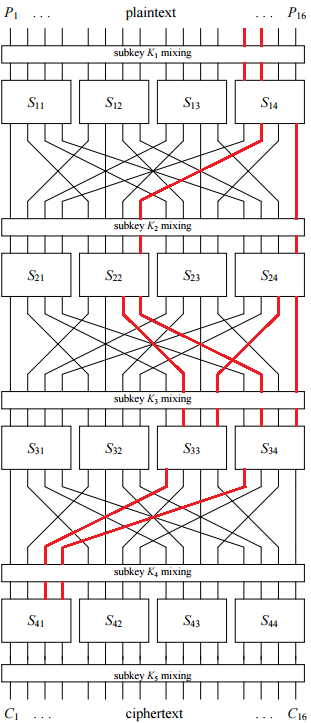
\includegraphics{12,12288}
  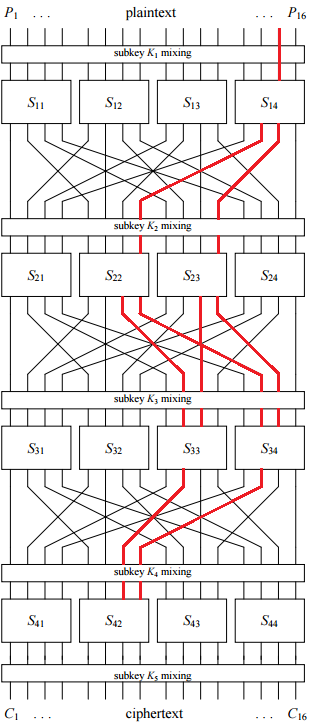
\includegraphics{13,768}
  \\ 
  \hspace{1cm}
  The diagrams above demonstrate the path through the substitution-permutation network undertaken to crack the first 8 bits of the subkey, using the differential pairs \lstinline{(12, 12288)} and \lstinline{(13, 768)} respectively.
  \clearpage
  
  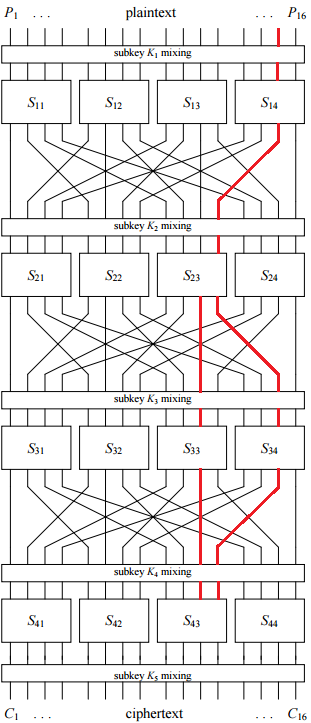
\includegraphics{2,48}
  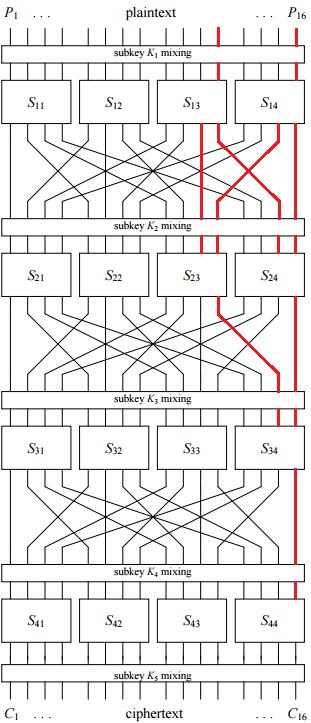
\includegraphics{17,1}
    \\ 
  \hspace{1cm}
  The diagrams above demonstrate the path through the substitution-permutation network undertaken to crack the last 8 bits of the subkey, using the differential pairs \lstinline{(2, 48)} and \lstinline{(17, 1)} respectively.
  \clearpage

  \section{Blockattack.py}\label{app:blockattack}
  \lstinputlisting[language=Python]{../part2/block_attack.py}
\end{appendices}
\clearpage
\bibliographystyle{IEEEtranSN}
\bibliography{references}
\end{document}
